\subsection{Aplikácia - Passer}
\label{passer}
Na základe analyzovaných myšlienok sme vyvinuli aplikáciu nazvanú Passer. Je určená pre používateľov operačného systému iOS, teda ide o telefóny značky Apple. 

Hneď po naštartovaní Passera je používateľovi ponúknutá možnosť vytvoriť nové heslo: 

\begin{figure}[H]
  \centering
  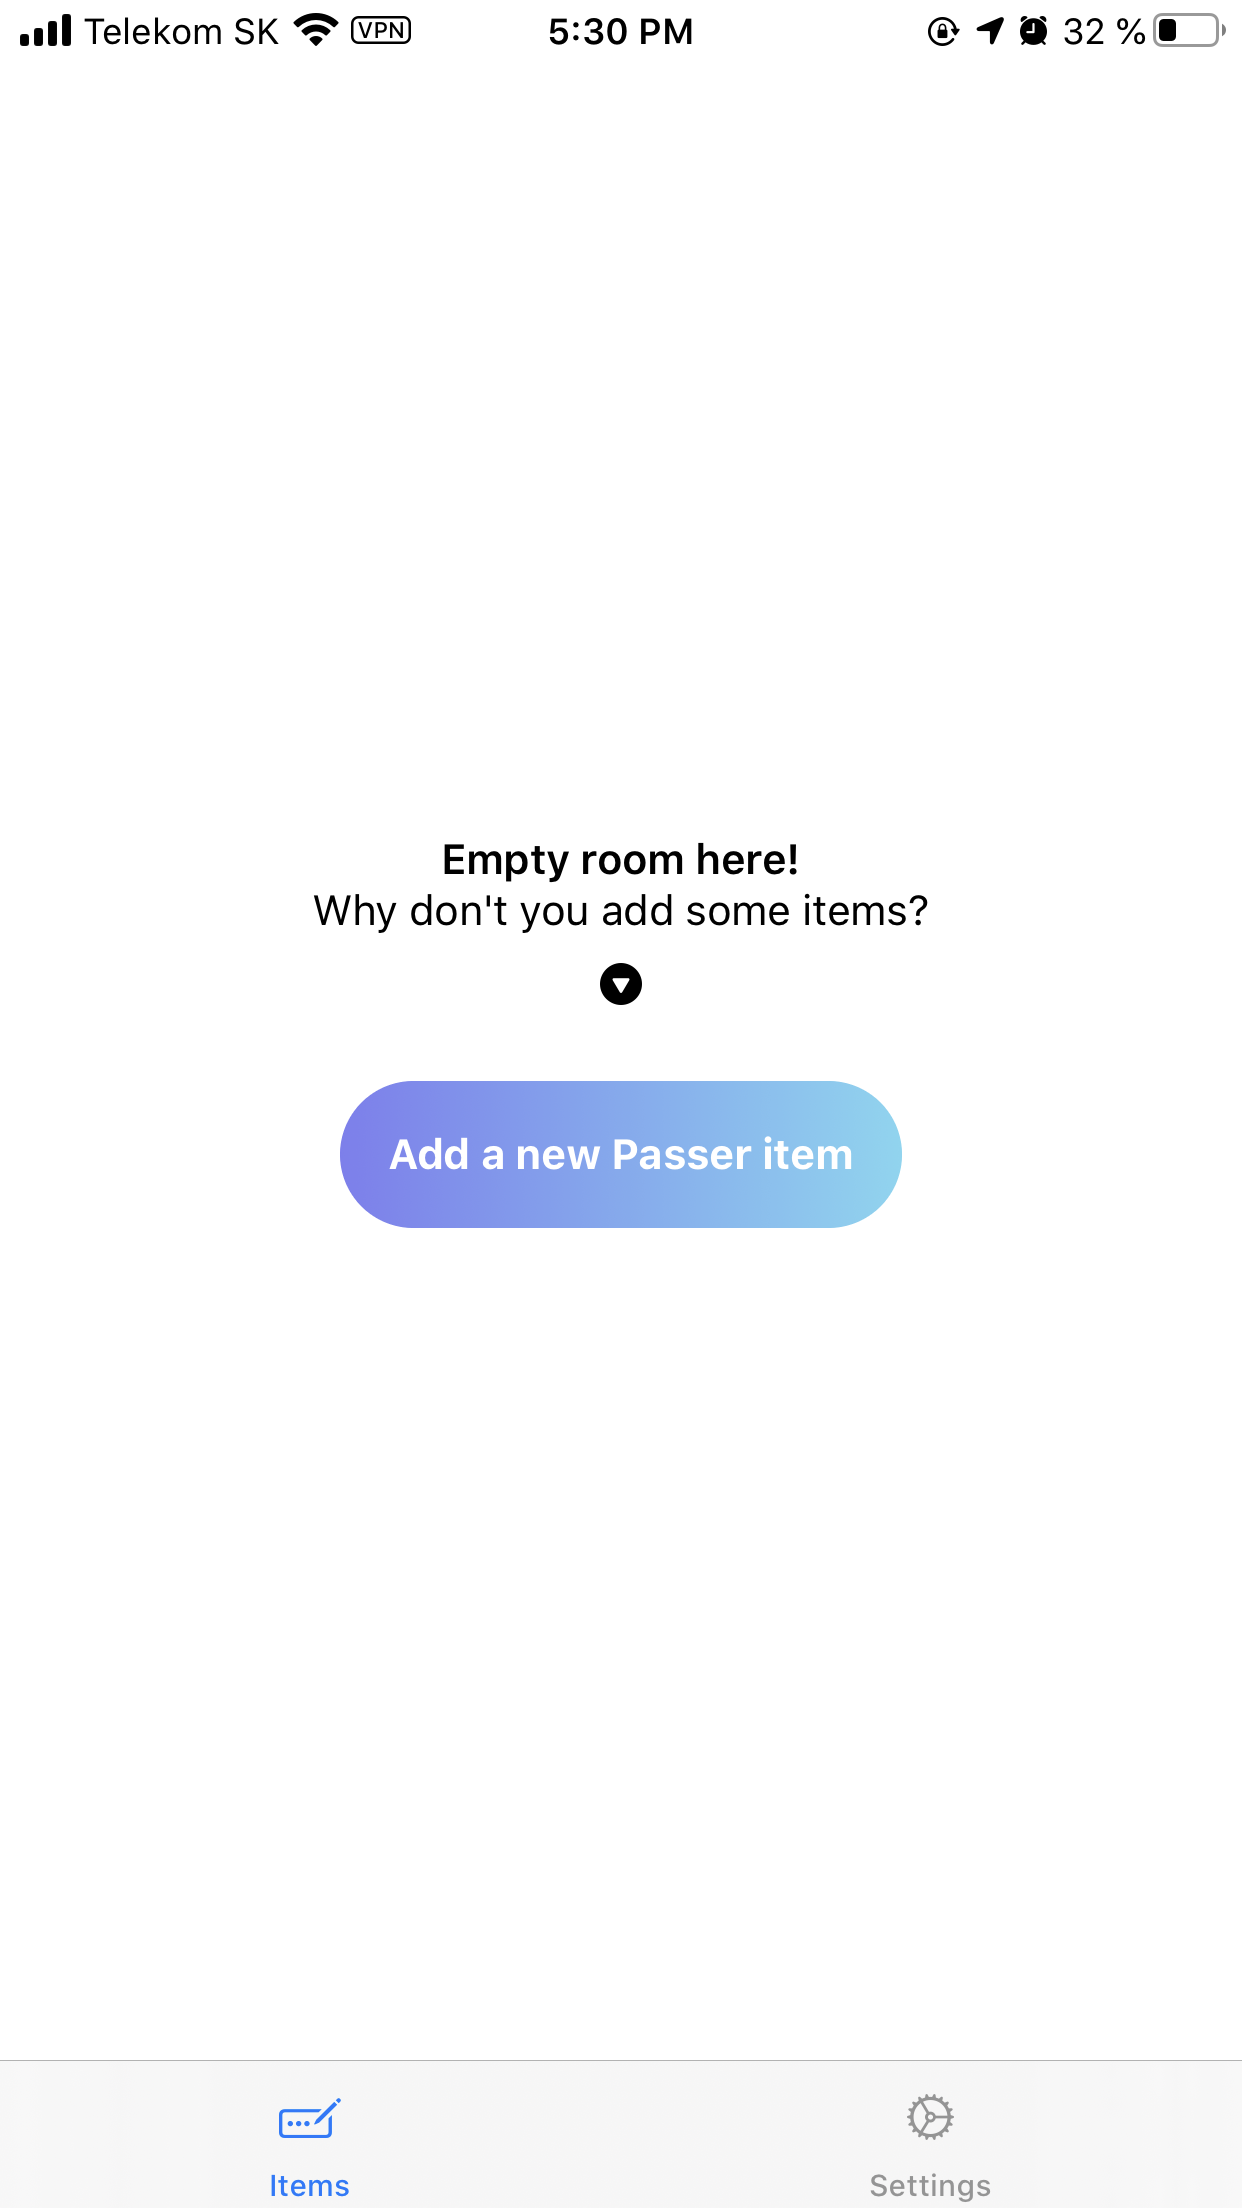
\includegraphics[width=7cm]{img/passer1.PNG}
  \caption{Úvodná obrazovka po prvom spustení.}
  \label{passer1}
\end{figure}

Po kliknutí na tlačidlo \textit{Add a new Passer item} si môže používateľ vytvoriť novú položku: 

\begin{figure}[H]
  \centering
  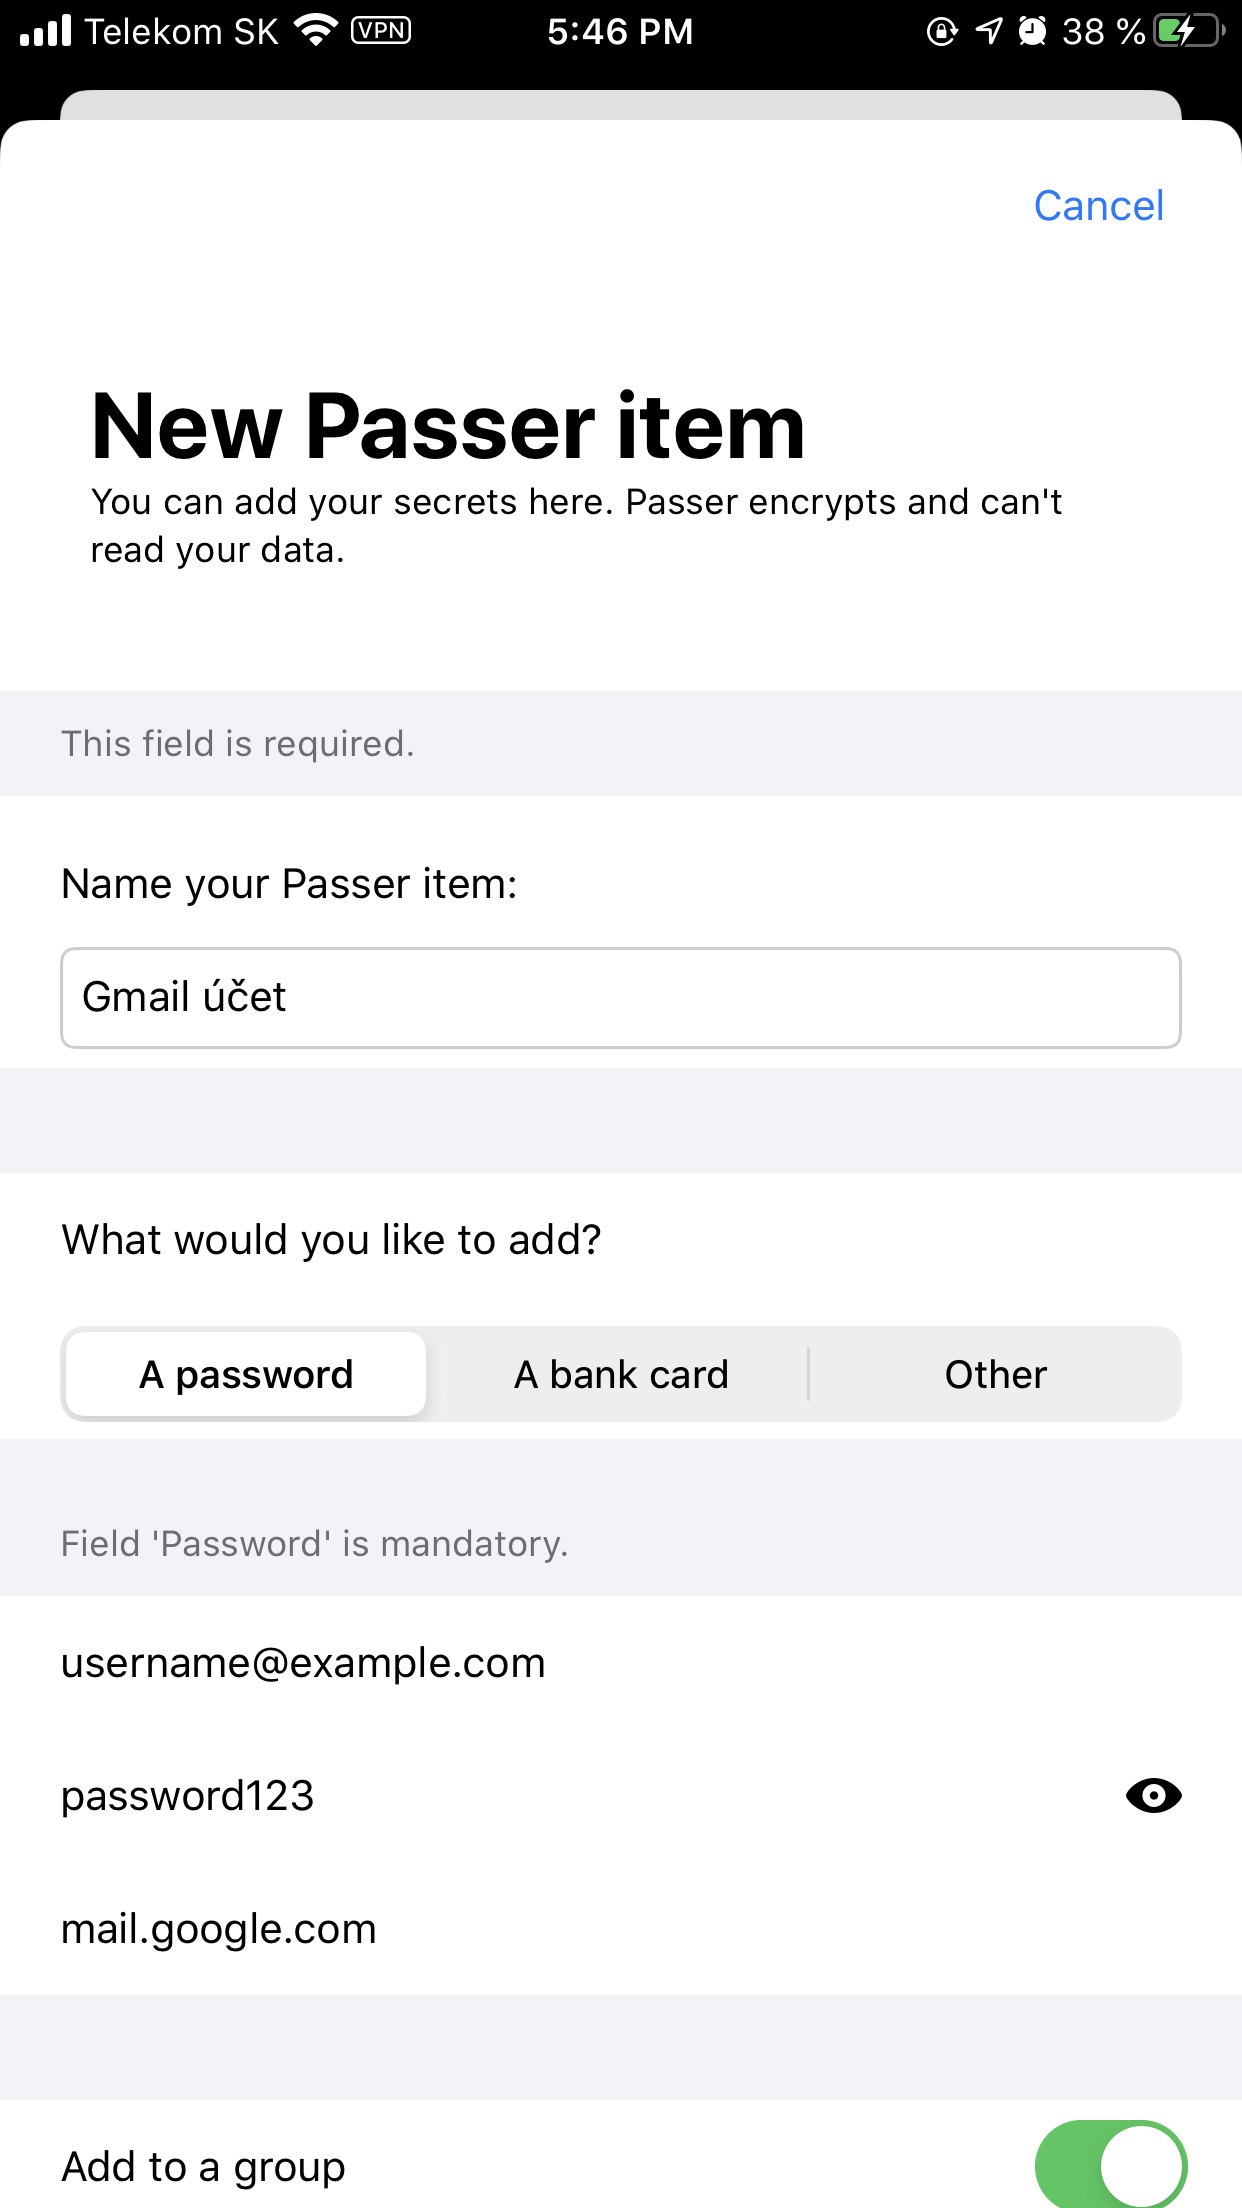
\includegraphics[width=7cm]{img/passer2.PNG}
  \caption{Pridávanie novej položky.}
  \label{passer2}
\end{figure}

Používateľ má k dispozícii mnohé atribúty. Môže dať názov svojej položke. Potom si vyberie o akú položku ide. Passer ponúka tri možnosti: heslo, banková karta, iné. V závislosti od výberu sa menia textové polia nižšie. Na \figurename{ \ref{passer2}} je zvolená možnosť \textit{A password}, takže v tomto prípade ide o heslo. Používateľovi sa dostavia k dispozícii tri textové polia:
\begin{itemize}
    \item[-] Email alebo používateľské meno
    \item[-] Heslo
    \item[-] Webová stránka
\end{itemize}

Môžeme vidieť, že v textovom poli s heslom je napravo malá ikona s okom. Používateľ môže na ňu klikať a tým sa heslo skryje za znaky bodiek alebo zobrazí ako plaintext. V kóde reprezentuje tlačidlo oka akýsi prepínač UI elementov vo frameworku SwiftUI jazyka Swift. V závislosti od stlačenia oka sa striedajú \texttt{TextField} a \texttt{SecureField}, ktoré zdieľajú svoj obsah v jednej premennej. Na rozdiel od \texttt{TextField} \cite{textfield_swiftui}, ktorý je len klasickým textovým poľom ukladajúcim jej obsah do nejakej premennej, \texttt{SecureField} \cite{securefield_swiftui} svoj obsah ukrýva.

Pri testovaní Passera sme pri tomto bezpečnom textovom poli spozorovali zaujímavé správanie. Po vytvorení snímky obrazovky sme zistili, že ani samotné bodky, ktoré nahrádzajú plaintext v \texttt{SecureField} neboli na screenshote. Jednoducho zmizli.

Nasledujúci obrázok zobrazuje nasledujúce možnosti pri pridávaní hesla. Prepínač \textit{Add to a group} umožňuje používateľovi zaradiť položku do skupiny. Passer poskytuje kategórie \textit{Personal} (osobné) a \textit{Work} (pracovné). Mimo tohto výberu si môže používateľ vybrať, či bude daná položka zaradená do jeho obľúbených. 

\begin{figure}[H]
  \centering
  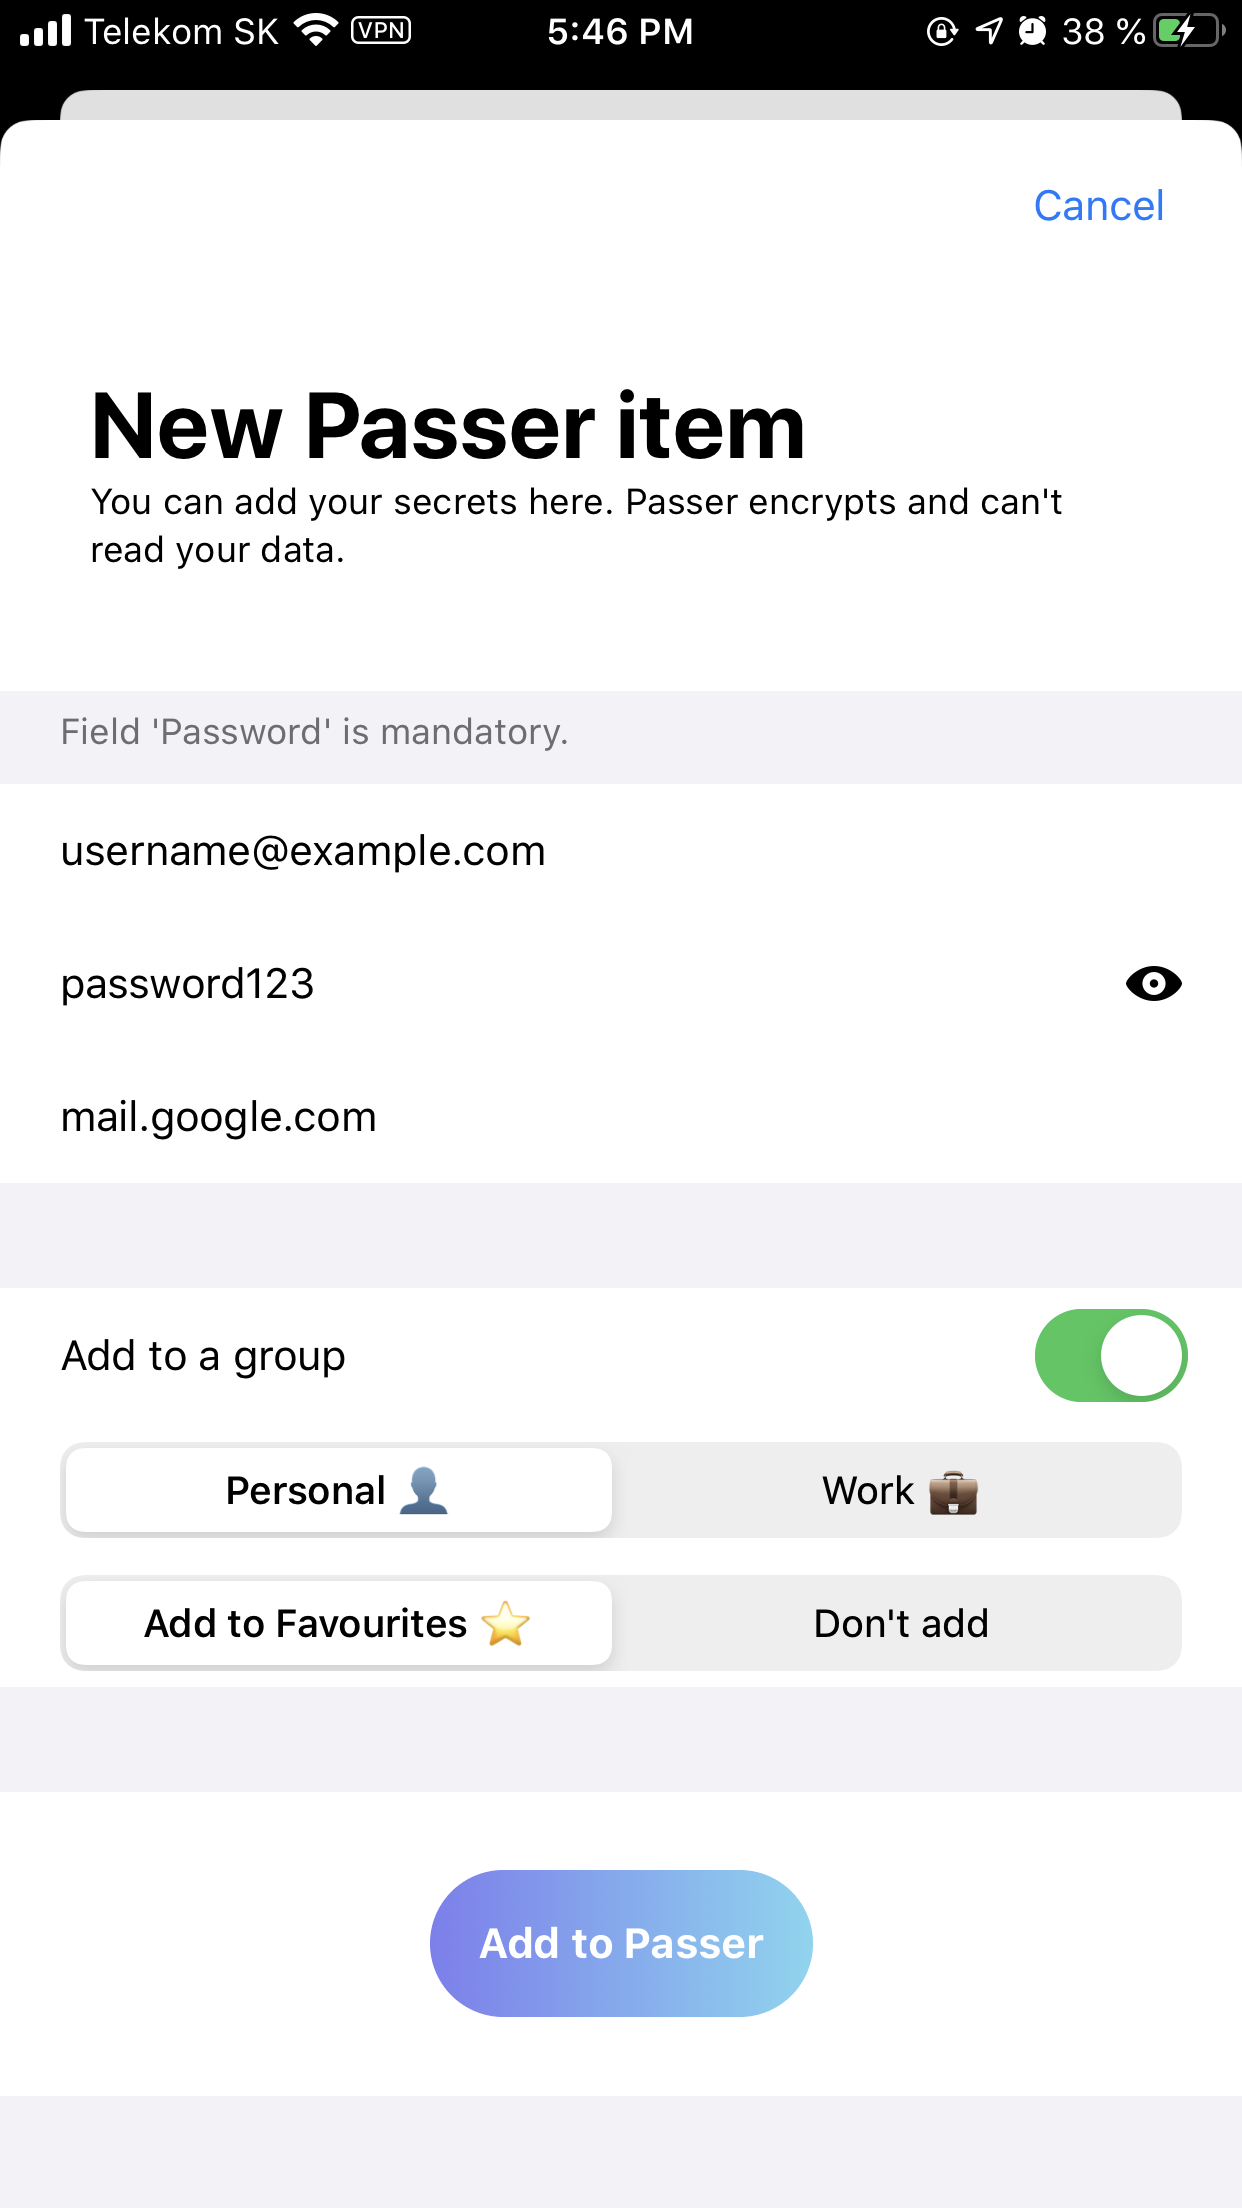
\includegraphics[width=7cm]{img/passer3.PNG}
  \caption{Pridávanie novej položky do skupín.}
  \label{passer3}
\end{figure}

Keď je používateľ so všetkým spokojný, kliknutím na \textit{Add to Passer} sa položka úspešne pridá medzi ostatné položky.

Takýmto spôsobom sme vytvorili ešte ďalšie dve položky, všetky typu heslo. Po týchto úkonoch má používateľ v Passerovi už tri položky. Nasledujúci obrázok ukazuje úvodnú obrazovku Passera, ak má používateľ aspoň jednu položku:\footnote{obrazovka z \figurename{ \ref{passer1}} sa už neukáže po ďalšom spustení.} 

\begin{figure}[H]
  \centering
  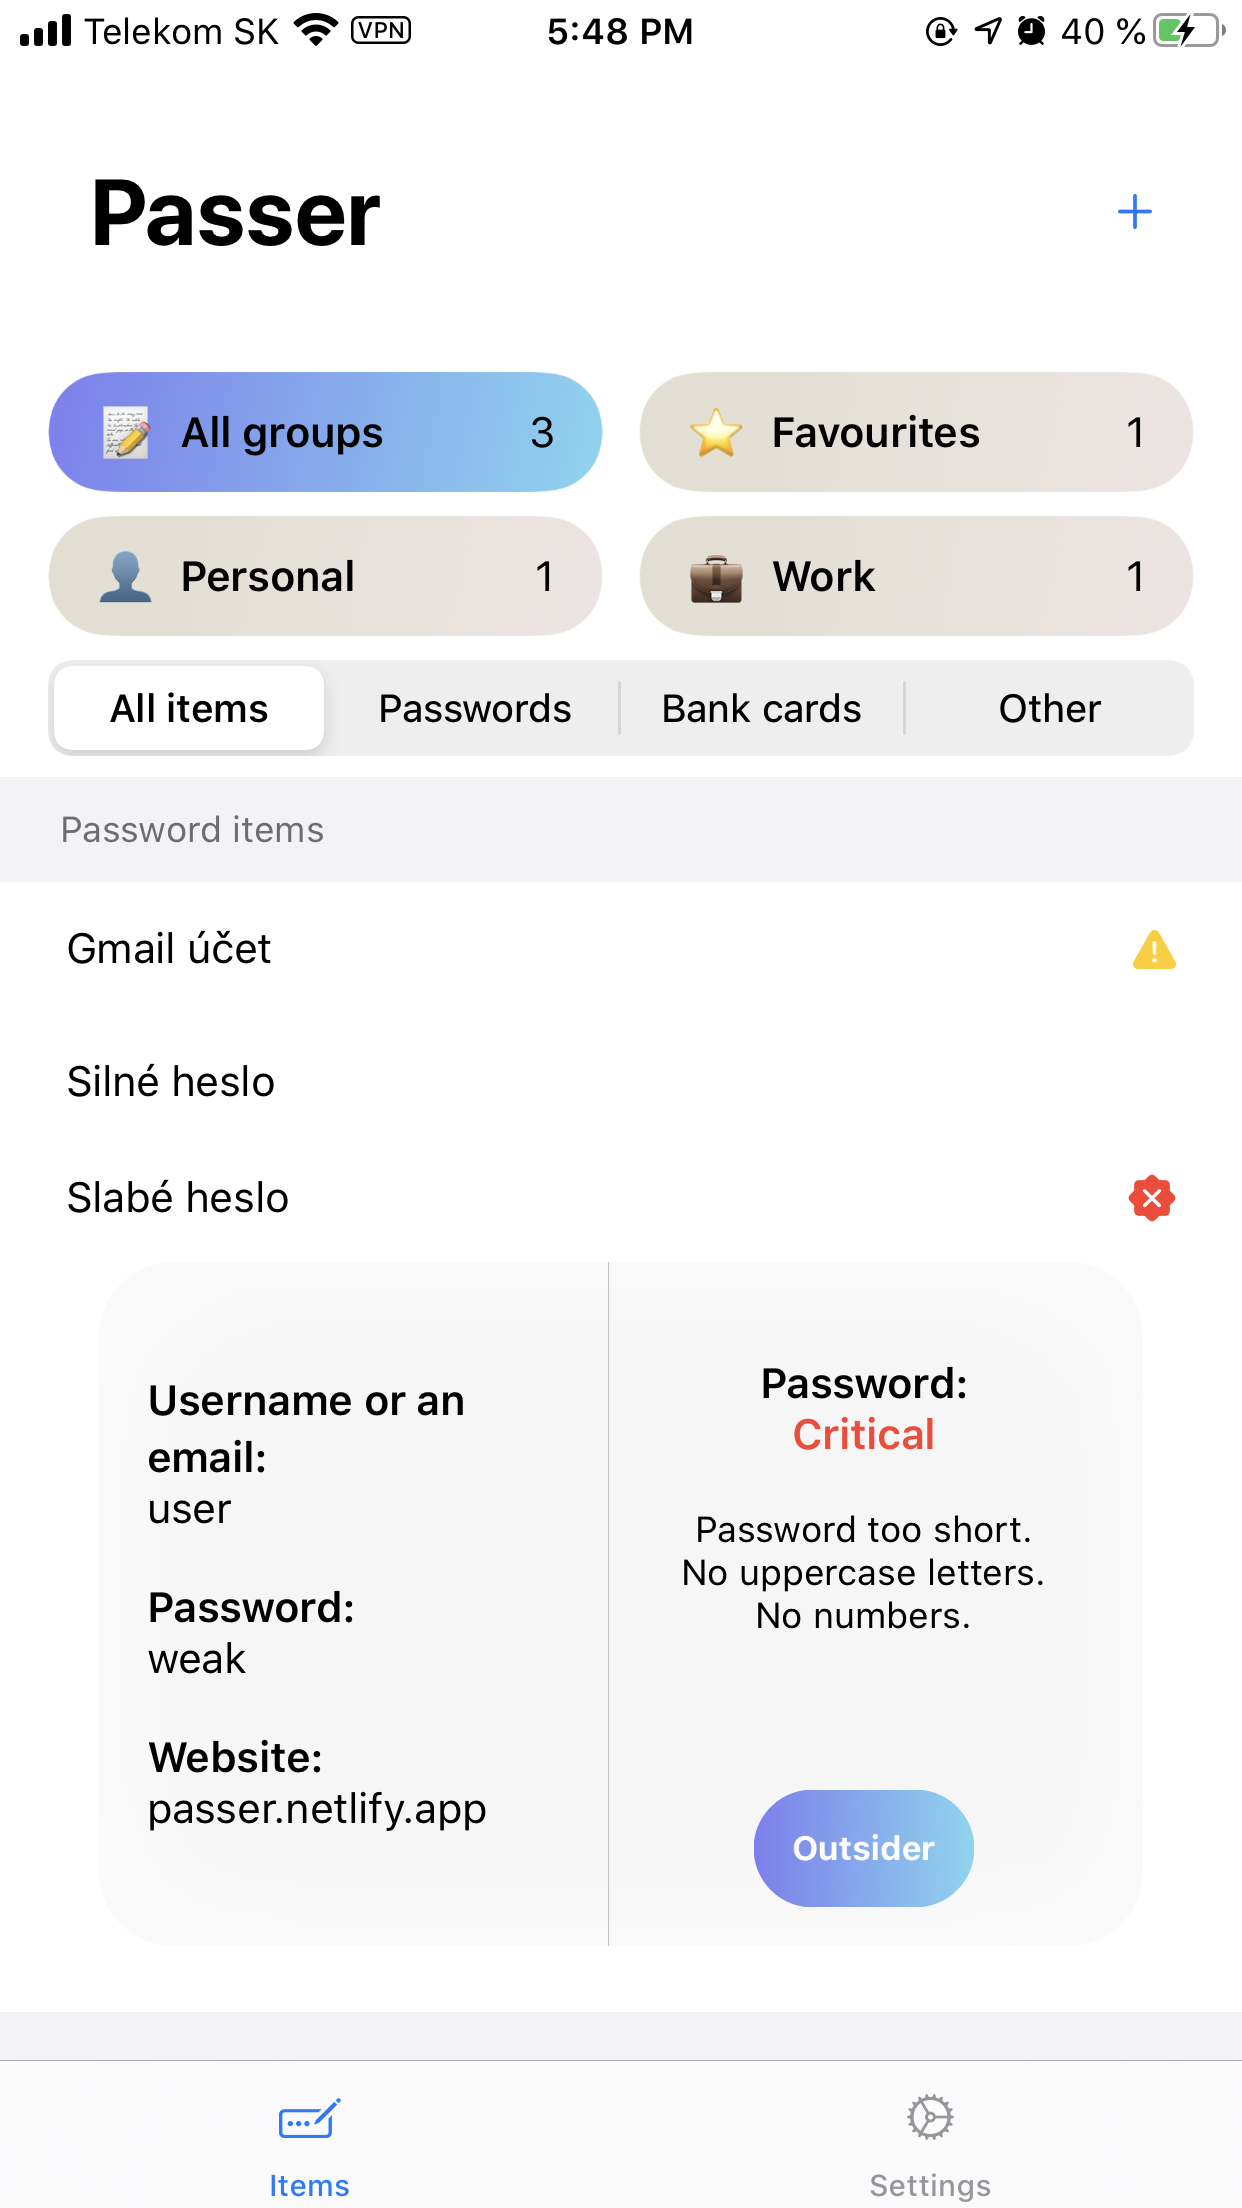
\includegraphics[width=7cm]{img/passer4.PNG}
  \caption{Úvodná obrazovka s heslami.}
  \label{passer4}
\end{figure}

\figurename{ \ref{passer4}} nám ukazuje tri heslá. Všimnime si ikonu žltého výkričníka pri položke \textit{Gmail účet} a červenú ikonu kríža pri položke \textit{Slabé heslo}. To je indikátor, ktorý hovorí, že heslo nie je dostatočne silné. Po kliknutí na jednu z položiek sa nám o nej rozbalia ďalšie informácie.

Screenshot ukazuje, že používateľ klikol na \textit{Slabé heslo}, takže sa zobrazili aj dodatočné informácie. Vidíme všetky tri atribúty, ktoré sme vypĺňali pri pridávaní novej položky do Passera. Napravo od týchto informácií vidíme červeným nápis \textit{Critical} (kritické). To znamená, že heslo je kriticky slabé. Passer nám vypísal aj dôvody. Sú až tri: Heslo je príliš krátke (minimálna dĺžka je osem znakov), heslo neobsahuje veľké písmená, heslo neobsahuje čísla.

V prípade žltého výkričníka je ohodnotenie \textit{Vulnerable} (zraniteľné). Heslo, ktoré je dostatočne silné nemá pri sebe žiadny indikátor (viď. položka \textit{Silné heslo}).

Logika vyhodnocovania je jednoduchá. Ak je heslo kratšie než osem znakov, alebo obsahuje iba malé písmená, iba veľké písmená alebo iba čísla, vyhodnotenie je \textit{Critical}. Tu sa vráťme k podkapitole \nameref{silahesla}, ktorá vysvetľuje prelomiteľnosť hesla. Tam sme hovorili, že ak aj použijeme kombináciu MP + VP + C (h3sL0), heslo je stále prelomiteľné pri offline útoku do sekundy. Preto je v tomto Passer vyhodnotenie prísne. Dĺžku hesla považuje za rovnako dôležitú ako kombináciu MP + VP + C. Keby bolo heslo h3sL0 v Passeri, stále by malo \textit{Critical} ohodnotenie.

Ak heslu chýbajú čísla, alebo veľké, alebo malé písmená, ale inak všetko ostatné je v poriadku, vyhodnotenie je \textit{Vulnerable}. Také heslo nie je vystavené veľkému nebezpečiu, ale stále je múdre predísť tomuto stavu.

Rovnaké indikátory fungujú pri bankových kartách v Passeri. Samozrejme, tu nevieme hodnotiť silu hesla, ale vieme kontrolovať dátum expirácie karty. Ikona žltého výkričníka symbolizuje, že karta expiruje čoskoro. Ikona červeného kríža hovorí, že karta už expirovala. Absencia ikony znamená, že je všetko s kartou v poriadku.

Všimnime si horný panel na \figurename{ \ref{passer4}}. Obsahuje rôzne filtre, na základe ktorých sa mení zobrazenie položiek nižšie. 

Panel začína filtrom na skupiny. Počas procesu vytvárania novej položky sme ukázali, že vieme pridávať položky do skupín a/alebo medzi obľúbených položky. Predvolená selekcia je zobrazenie všetkých skupín (\textit{All groups}).

Nižšie vidíme filter na typy položiek. Opäť sa odvoláme na proces vytvárania novej položky. V závislosti od voľby typu položky sa nám zobrazili korešpondujúce textové polia. Predvolená selekcia je zobrazenie všetkých typov (\textit{All items}).

Po aplikovaní filtrov \textit{Favourites} a \textit{Passwords} vyzerá úvodná obrazovka s heslami nasledovne:

\begin{figure}[H]
  \centering
  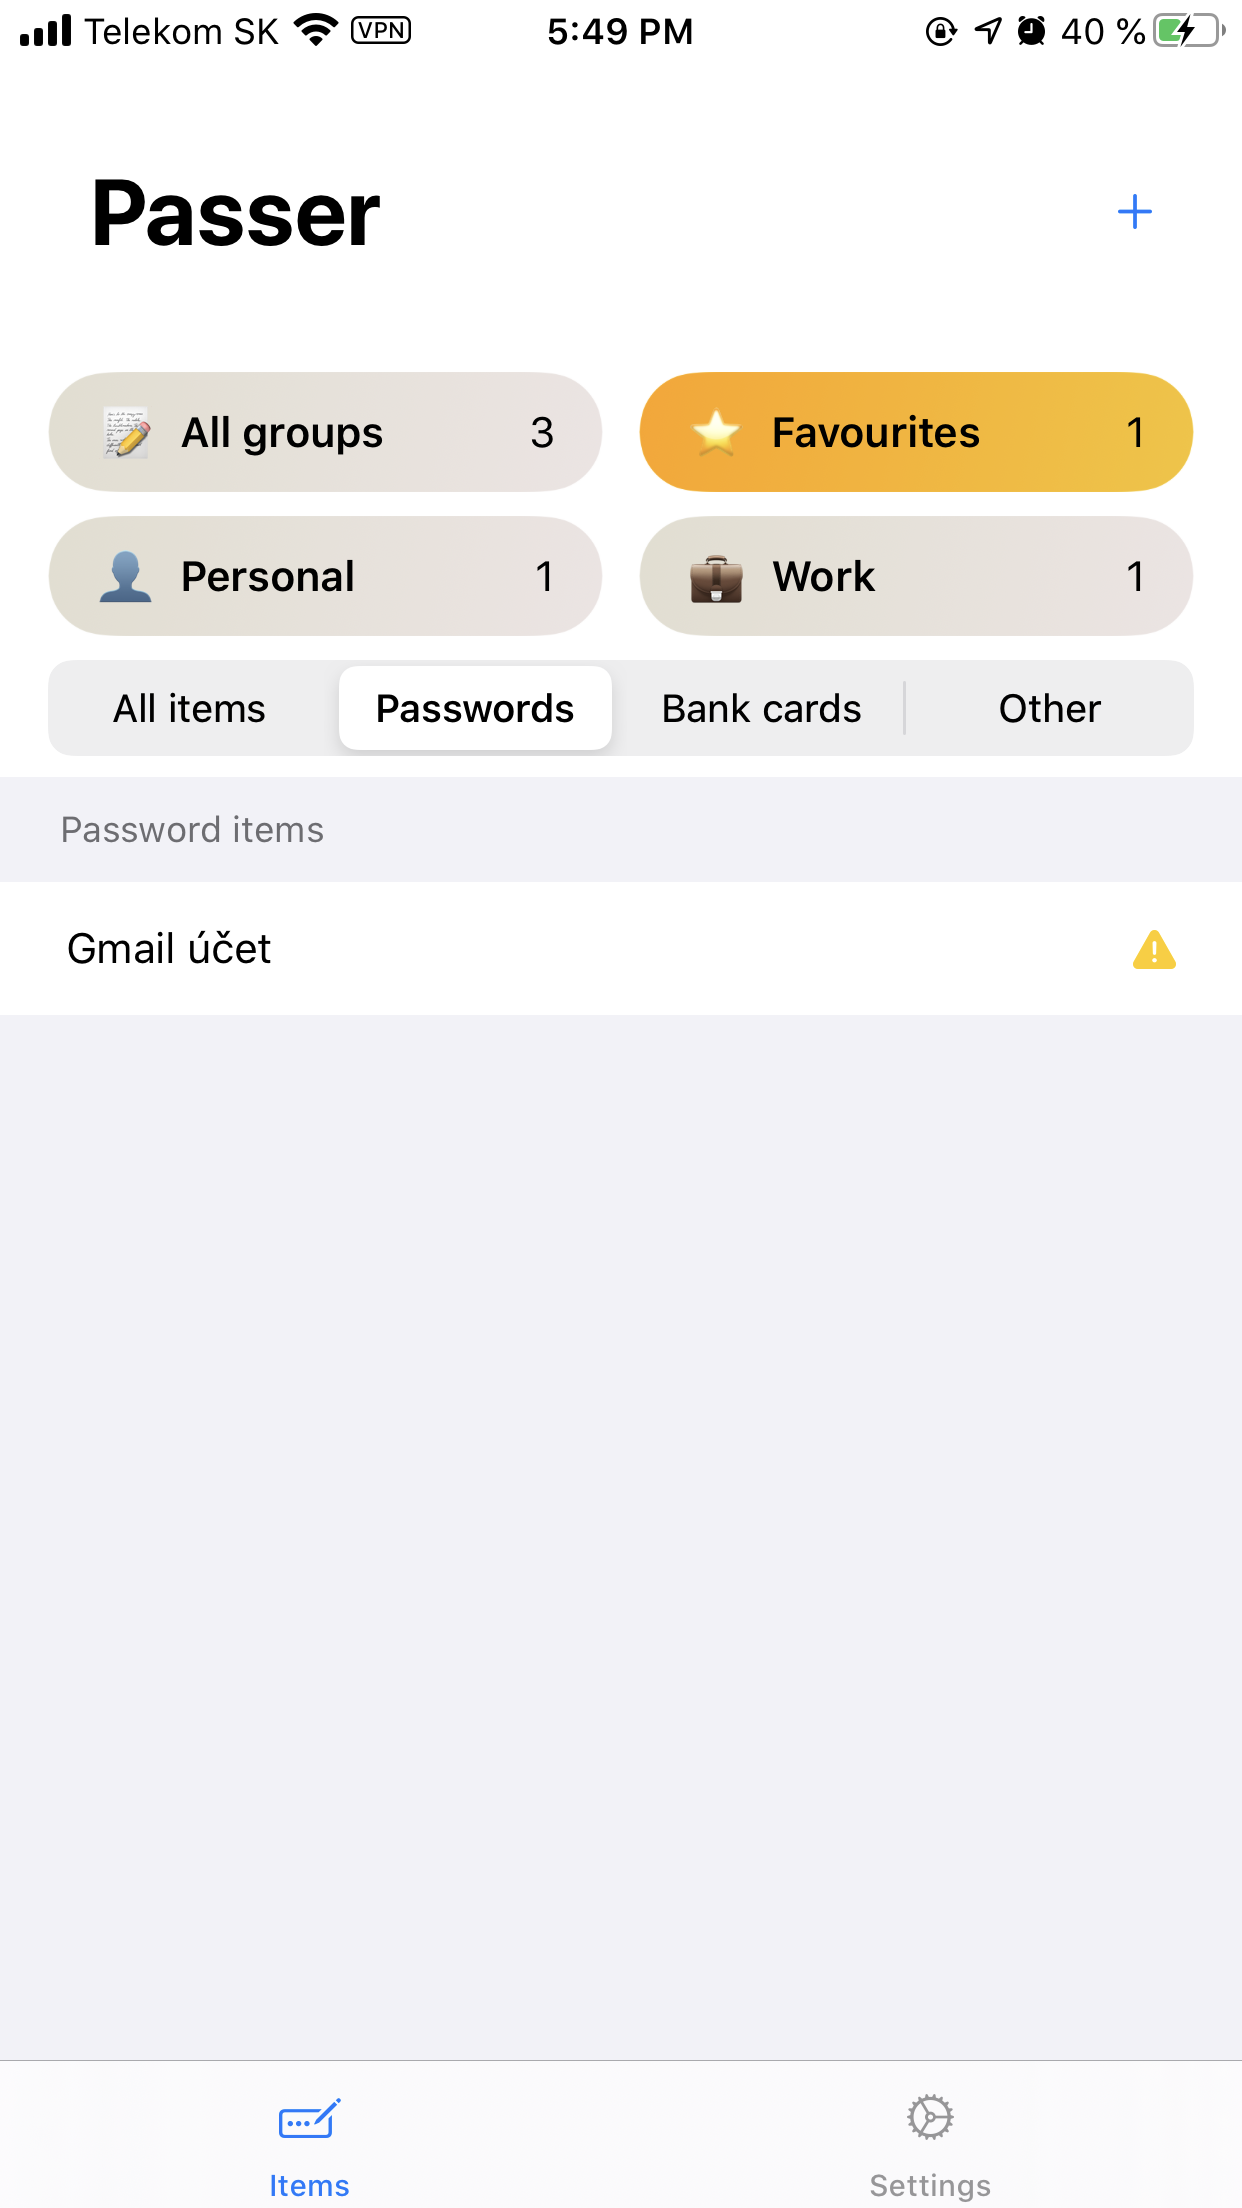
\includegraphics[width=7cm]{img/passer5.PNG}
  \caption{Úvodná obrazovka s heslami po aplikovaní filtrov.}
  \label{passer5}
\end{figure}

\subsubsection{Outsider}
Prejdime k hlavnému bodu celej aplikácie. Funkcionalita s názvom \textit{Outsider} dokáže akúkoľvek položku poslať cez server na webstránku. Zároveň pre používateľa vytvorí jednorázovú verifikáciu, ktorá expiruje po dvoch minútach alebo po jej použití. 

Proces začína kliknutím na položku v úvodnej obrazovke (viď \figurename{ \ref{passer4}}). Môžeme vidieť, že napravo od detailov položky je prítomné tlačidlo \textit{Outsider}. Po kliknutí je používateľ presmerovaný na nasledujúcu obrazovku:

\begin{figure}[H]
  \centering
  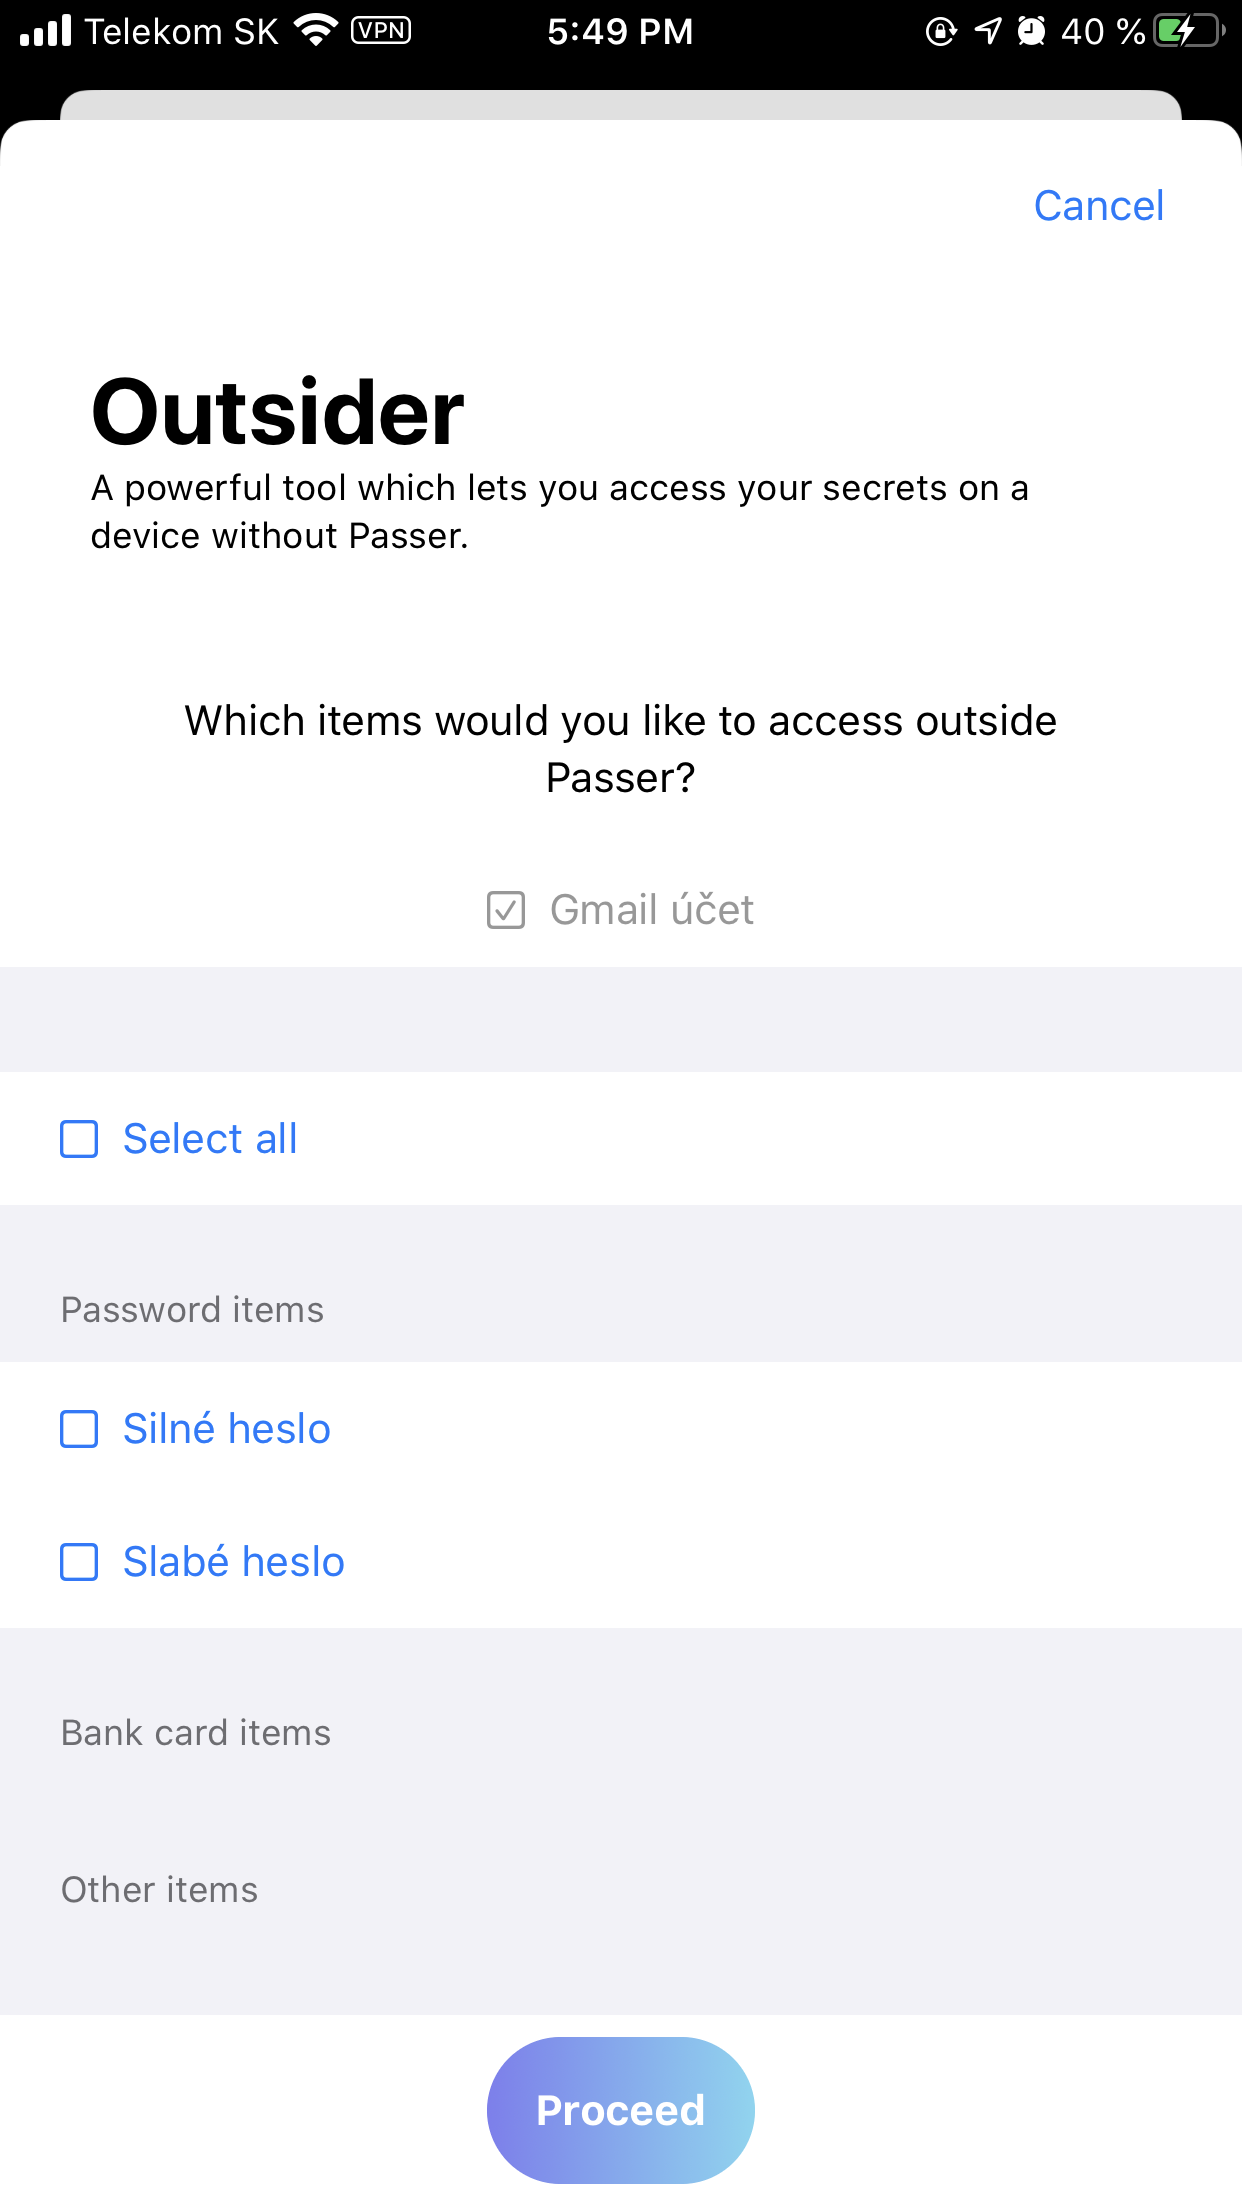
\includegraphics[width=7cm]{img/passer6.PNG}
  \caption{Outsider - výber položiek.}
  \label{passer6}
\end{figure}

Podľa toho, z akej položky klikneme na tlačidlo \textit{Outsider} sa mení správanie na obrázku vyššie. V danom prípade vidíme, že je predvolene zvolený \textit{Gmail účet}, pretože sme z tejto položky prešli na Outsider. Nedá sa odznačiť, čo symbolizuje aj šedá farba. 

Na druhej strane, v dolnej polovici obrazovky môžeme pridať ľubovoľný počet ďalších z našich položiek, ktoré sa odošlú spolu s \textit{Gmail účet}. Vidíme možnosť \textit{Select all}, ktorá označí všetky položky. Po kliknutí sa možnosť zmení na \textit{Deselect all}, aby mohol používateľ odznačiť všetko v prípade, že by zmenil názor. Je dôležité povedať, že po kliknutí na \textit{Deselect all} sa neodznačí položka, z ktorej bol používateľ presmerovaný na obrazovku Outsidera. Z tohto je zrejmé, že Outsider nikdy nepošle prázdne pole položiek na server. Pod spomínaným tlačidlom už vidíme jednotlivé položky, ktoré sú tiež tlačidlami. Ich stlačením sa daná položka pridá, respektíve odoberie zo zoznamu položiek na odoslanie.

Ak je používateľ spokojný s výberom, postupuje na ďalšiu obrazovku kliknutím na tlačidlo \textit{Proceed}.

\begin{figure}[H]
  \centering
  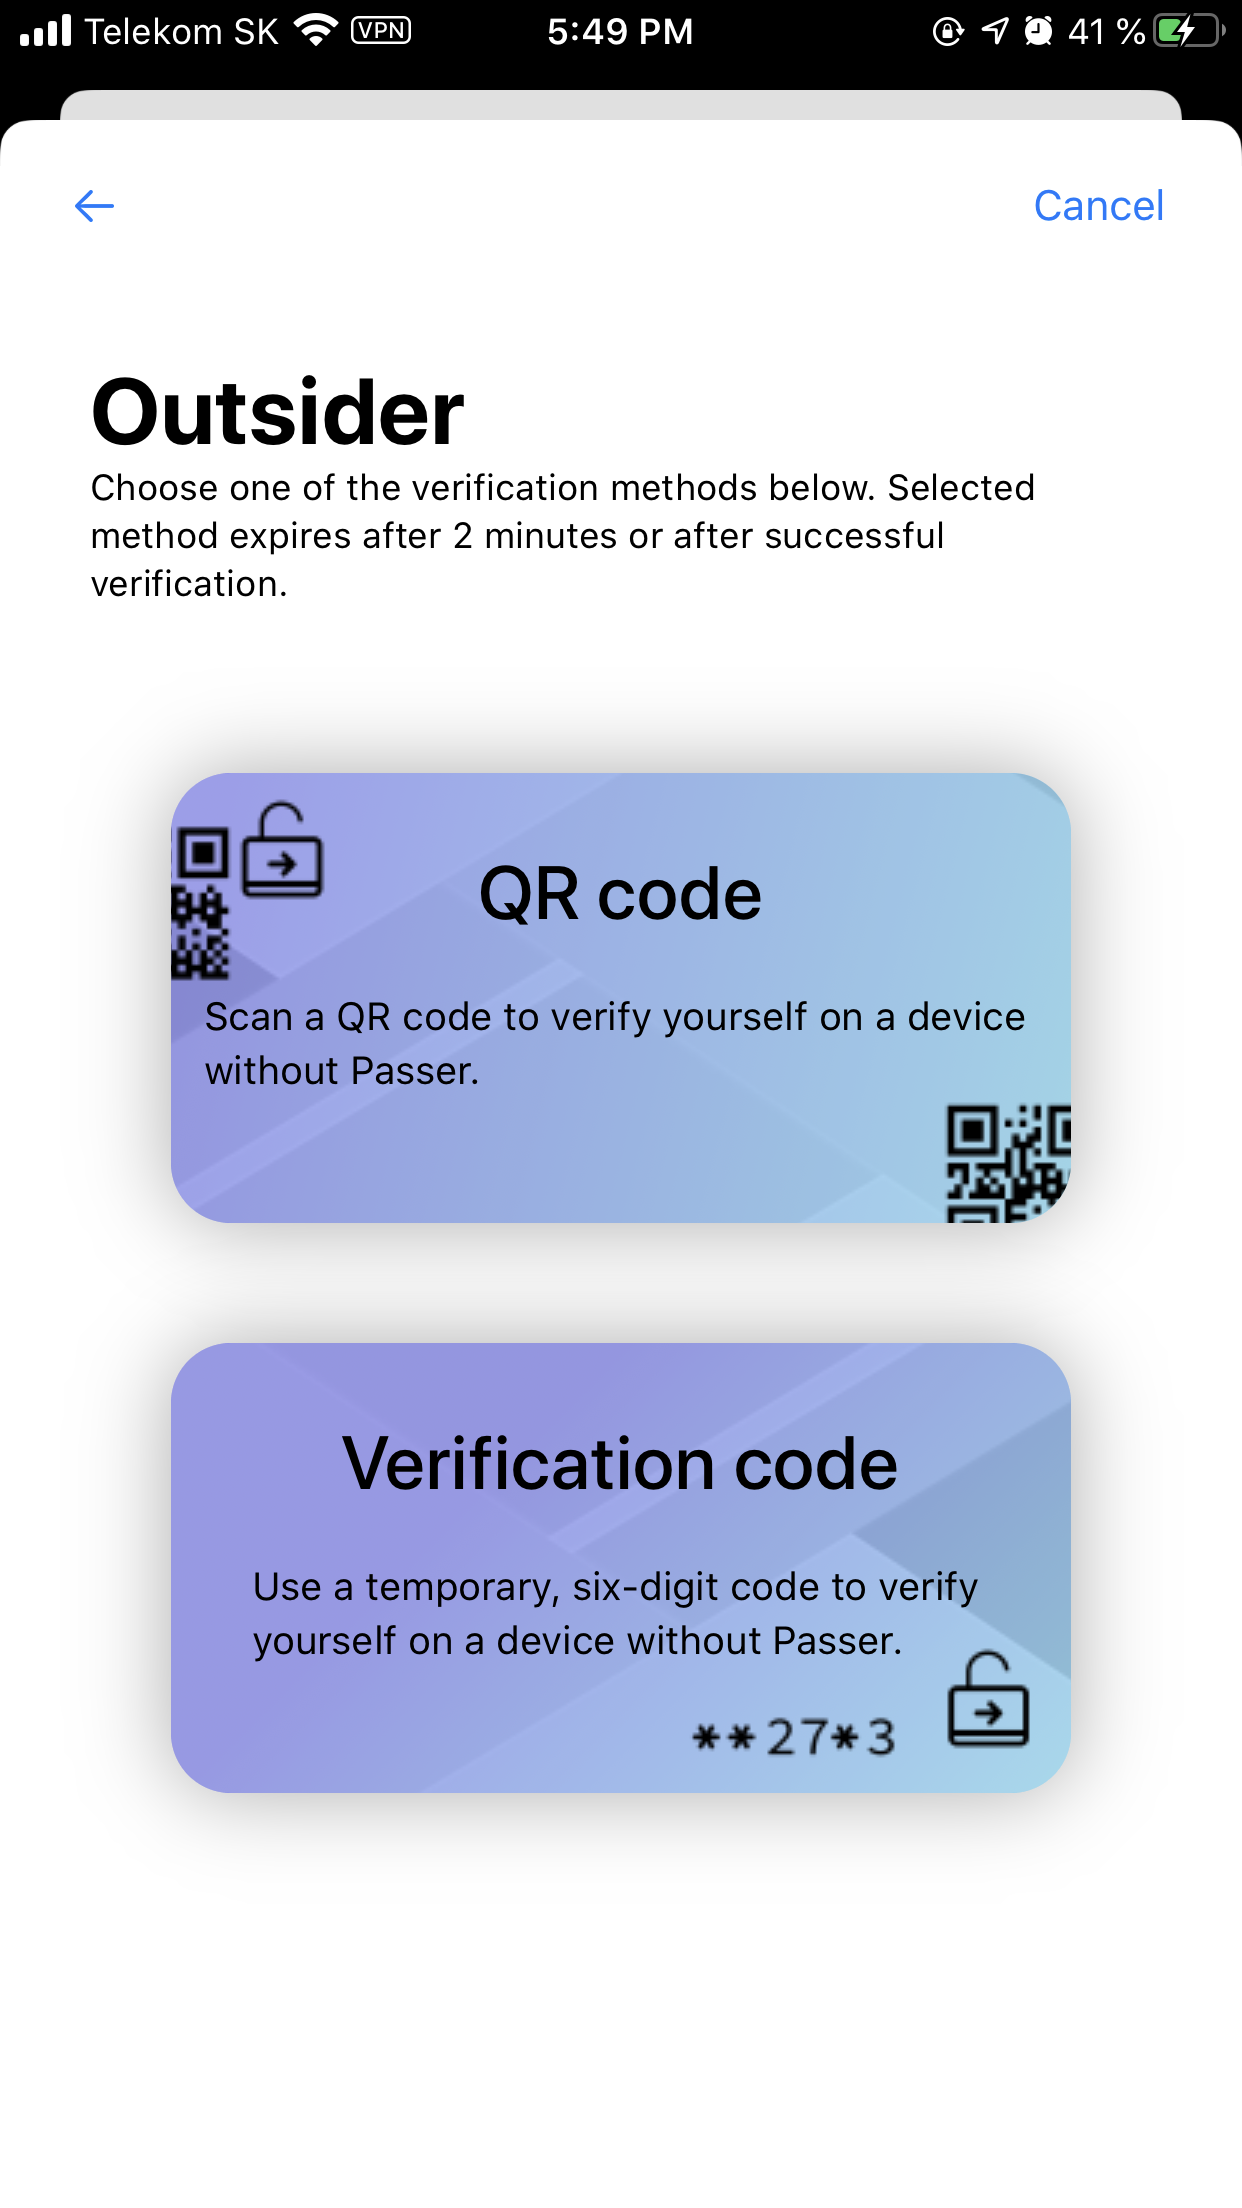
\includegraphics[width=7cm]{img/passer7.PNG}
  \caption{Outsider - výber typu verifikácie.}
  \label{passer7}
\end{figure}
Položky na odoslanie sú pripravené. Teraz nasleduje výber typu verifikácie.

Prvá z možností je nasnímanie QR kódu. Využijeme fakt, že Passer je určený pre zariadenia iPhone. Každý model má kameru. Môže byť použitá na nasnímanie QR kódu na webstránke.

Druhá možnosť je použiť šesťciferný kód, ktorý používateľ následne zadá na webstránke. Ak je kód správny, webstránka sprístupní odoslané heslá používateľovi.

\begin{figure}[H]
  \centering
  \includegraphics[width=7cm]{img/passer8.PNG}
  \caption{Outsider - QR kód.}
  \label{passer8}
\end{figure}

Po kliknutí na možnosť verifikácie pomocou QR kódu sa používateľovi v dolnej časti zobrazí obraz, ktorý vidí kamera. Spolu s ním dostane inštrukcie, na akú stránku má ísť a čo má robiť. 

Proces, ktorý sa deje na pozadí vysvetlíme až v sekcii \nameref{vzajomne_interakcie}, nakoľko tento proces je veľmi špecifický. A to z dôvodu, že táto verifikácia interaguje aj s webstránkou, aj so serverom.

\begin{figure}[H]
  \centering
  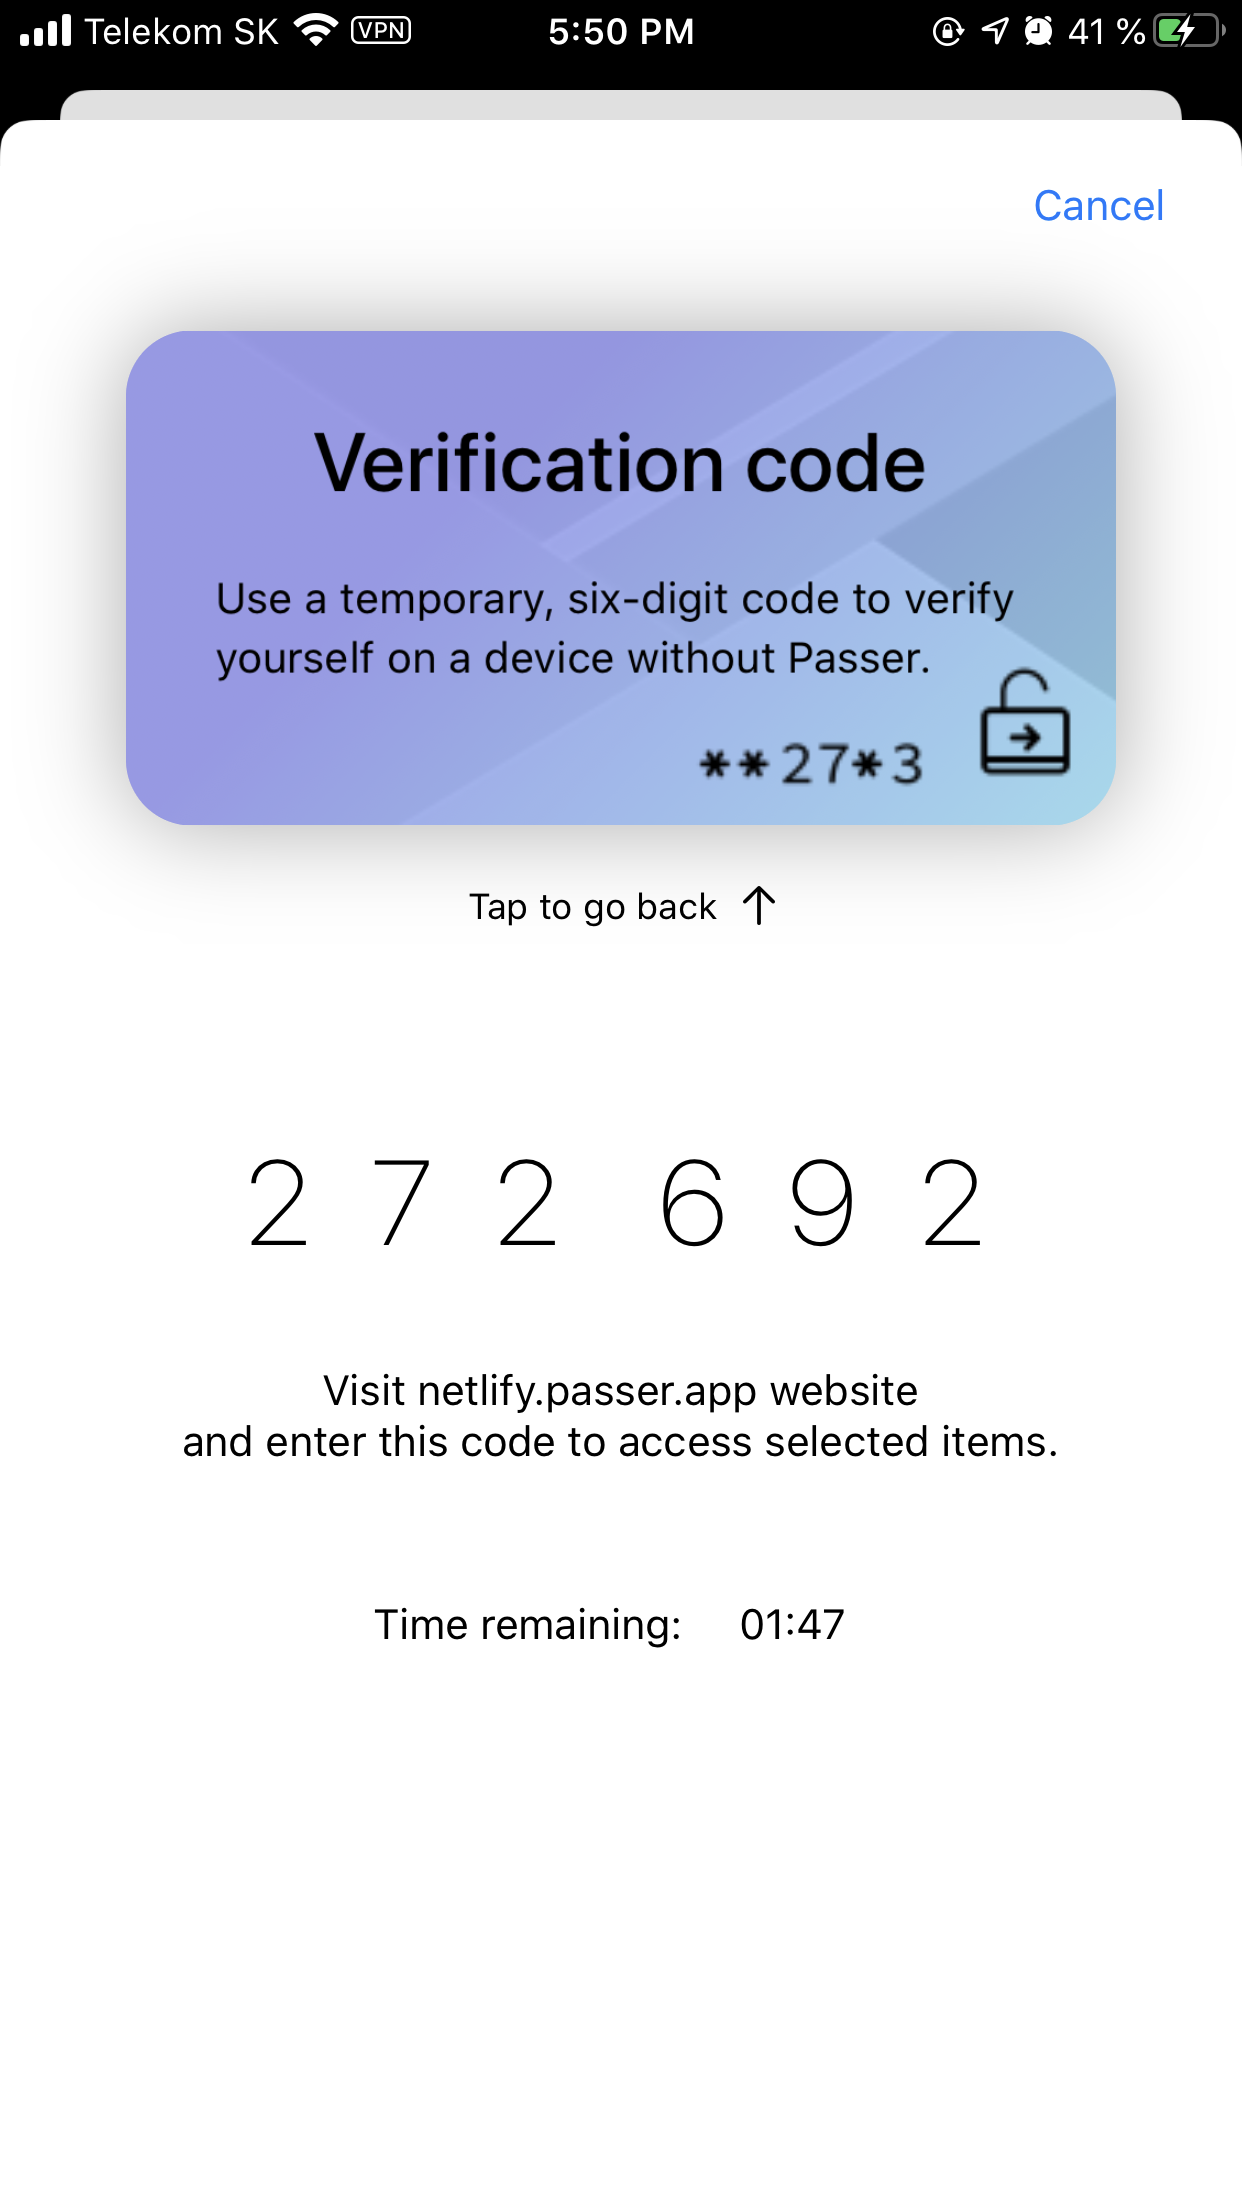
\includegraphics[width=7cm]{img/passer9.PNG}
  \caption{Outsider - Šesťciferný kód.}
  \label{passer9}
\end{figure}

Pozrime sa na to, ako príde k tomu, že používateľ obdrží jednorázový, šesťciferný kód. Po kliknutí na túto možnosť sa na pozadí vytvorí inštancia štruktúry \texttt{SixdigitAuth}, ktorá vyzerá v kóde nasledovne:
\newline
\begin{lstlisting}[language=Swift, basicstyle=\small]
struct SixdigitAuth: Codable {
    fileprivate let deviceID: String
    let sixdigitCode: String?
    let passwordItems: [PasswordItem]?
    let bankCardItems: [BankCardItem]?
    let otherItems: [OtherItem]?
    let timestamp: Date?
}
\end{lstlisting}
\leavevmode\newline

Atribút \texttt{deviceID} je generovaný iOS zariadením. Každé iOS zariadenie má jedinečné identifikačné číslo \cite{iOS_id}. Tento atribút je dôležitý a to preto, aby na serveri nemal jeden používateľ dva rôzne šesťciferné kódy. Ak počas dvoch minút používateľ zopakuje proces generovania kódu, na serveri nový kód prepíše ten starý. Toto opatrenie zvyšuje bezpečnosť. Keby používateľ neustále generoval nové a nové kódy (toto všetko v rozmedzí dvoch minút), tak by existovalo oveľa viac možností, ako sa na webstránke dostať k súkromným údajom daného používateľa. Týmto ošetrením má používateľ na serveri najviac jednu verifikáciu, ktorá je správna.

\texttt{sixdigitCode} je String, ktorý vznikol pospájaním šiestich, náhodne vygenerovaných čísiel Passerom. Atribúty \texttt{passwordItems}, \texttt{bankCardItems} a \texttt{otherItems} sú polia, ktoré majú obsahovať položky rôznych typov na odoslanie. Polia môžu byť prázdne. Posledný atribút \texttt{timestamp} vytvorí časovú pečiatku, kedy bola táto inštancia vytvorená. Podľa toho Passer vie, koľko času ostáva používateľovi do konca platnosti. Zobrazuje ho v \figurename{ \ref{passer9}} ako výsledok rozdielu \texttt{timestamp} a aktuálneho času. Túto kalkuláciu Passer vykonáva každú sekundu.\footnote{častejšie netreba, nakoľko čas sa zobrazuje v minútach a sekundách.}

Nad touto štruktúrou vykoná Passer serializáciu do dátovej štruktúry JSON, aby ju server vedel čítať. JSON je následne poslaný na server. V tomto momente Passer čaká na odpoveď. Ak je pozitívna, môže považovať vygenerovaný kód za použiteľný. Až v tomto momente je zobrazený používateľovi na obrazovke. Detailnejší rozbor poskytujeme v \nameref{vzajomne_interakcie}.
